\chapter{Ausgangsszenario}

\section{Anforderungen}
\label{Anforderungen}

% kartografisches Produkt
Aktuelle Möglichkeiten der Datenerfassung über Sensoren und moderne Probenahmegeräte führen zu mehr und mehr Datensätzen, die für einen Landwirtschaftsbetrieb ausgewertet werden müssen. Darüber hinaus besteht die Notwendigkeit, Daten Jahresübergreifend und betriebsübergreifend auszuwerten, um pflanzenbauliche Zusammenhänge über statistische Methoden untersuchen zu können.
In den letzten 3 Jahren wurde beispielsweise nur zum Thema N-Versorgung\footnote{Stickstoffdüngung und -aufnahme} für einen Betrieb etwa 800 Datensätze mit 1,9 Mio Einträgen erfasst. Alle diese Daten haben einen räumlichen Bezug, sie müssen weiterverarbeitet, kartographisch aufbereitet und dargestellt werden.\\
Daraus ergeben sich verschiedenen Anforderungen an die Technologie, die für die Verarbeitung, Analyse und Darstellung verwendet wird:
\begin{itemize}
\item PostgreSQL mit PostGIS zum Datenimport und -export nutzbar
\item Gruppieren und Filtern mit geringer Laufzeit
\item parallele Berechnung\footnote{hier Statistik bzw. Geostatistik sowie Interpolation} über große Datenmengen mit geringer Laufzeit
\item Räumliche Berechnungen wie Verschneiden, Berechnen von Overlays
\item  Unterschiedliche Prinzipien der Kartengenerierung, hier dynamisches rendern aus dem Datenbestand zur Laufzeit oder dynamisches rendern bei Dateneingang wodurch vorgerenderte Karten bereitstehen % caches wirklich mit untersuchen? wenn ja in Schnittstellen aufnehmen
\item nutzbare Schnittstelle zur Darstellung mit dem \Gls{umn}
\end{itemize}

% TODO: ergänzen, dass Anforderungne von Ist-Stand und möglichen Verbesserungen herrühren

% Eventuell technische SIcht extra darstellen, um Eignung der Systeme besser herausarbeiten zu können

Konkret handelt es sich bei den Eingangsdaten um folgende:
\begin{description}
\item[Pflanzenbauliche Daten]\footnote{Sensoren, Bodenuntersuchung, \Gls{bonitur}, Logger} Punktdaten
\item[Basisdaten wie Feldgrenzen] Vektordaten
\item[Externe Satelliteninformationen und Multispektralanalysen] Rasterdaten
\end{description}

\subsection{Softwarequalität}
\label{softwarequalität}
%TODO: warum hier die qualitätsmerkmale
Qualitätsmerkmale sind nach DIN 9126\footnote{DIN 9126 wurde durch ISO/IEC 25000 ersetzt, jedoch sind beide nur proprietär verfügbar} in \cite{book:lehrbuchsoftware} S. 258 f. Funktionalität, Zuverlässigkeit, Benutzbarkeit, Effizienz, Änderbarkeit und Übertragbarkeit.
Diese Merkmale werden durch Qualitätskriterien für jeden Anwendungsfall konkretisiert.


Nachfolgend werden die Qualitätsmerkmale für diesen Anwendungsfall konkretisiert und darauf die zu untersuchenden aufgelistet.


Da die zu analysierenden Systeme eine Datenbank beinhalten, welche mit räumlichen Datentypen arbeitet, wurde die im Anhang C von \cite{book:objdbs} enthaltene Checkliste zur Auswahl eines \Gls{odbms} berücksichtigt.

\textbf{Funktionalität}\\
Das System stellt alle geforderten Funktionen mit den definierten Eigenschaften zur Verfügung.
\begin{description}
\item[Richtigkeit] Ergebnisse sind korrekt oder ausreichend genau. Die Ergebnisse sollen zu 99\% mit denen des Ist-Standes übereinstimmen.
\item[Interoperabilität] Es sind Schnittstellen zur Ein- und Ausgabe vorhanden. Dabei soll es sich um PostgreSQL Import sowie PostgreSQL und \Gls{umn} Export handeln.
\item[Funktionsumfang] Mindestens die benannte und essentielle Menge an Funktionalitäten wird bereitgestellt. Dazu zählt:
parallele Verarbeitung, Gruppierungs-, Filter-, Verschneidungs- sowie Overlayfunktionen, Geostatistik und Umrechnung zwischen Koordinatensystemen und -formaten. Außerdem sind vorhandene Datentypen und Schemaversionierung von Interesse.
\item[Ordnungsmäßigkeit] Die Implementation des Systems und dessen Funktionen erfüllt Normen, Vereinbarungen, gesetzliche Bestimmungen und andere Vorschriften. Hierzu ist zu nennen, dass besonders Berechnungsfunktionen nach mathematischen Gesetzen implementiert sein müssen. Konkret sind Berechnungen der räumlichen Verarbeitung nach anerkannten definierten Algorithmen durchzuführen.
\end{description}
\ \\
%
\textbf{Zuverlässigkeit}
\begin{quote}
Fähigkeit einer Software, ihr Leistungsniveau unter festgelegten Bedingungen über einen festgelegten Zeitraum bewahren.\footnote{\cite{book:lehrbuchsoftware} S. 259}
\end{quote}
Nutzung von Tools zur Überwachung und Konfiguration immanent.
\begin{description}
\item[Fehlertoleranz] Das System sollte auftretende Fehler des Tagesgeschäftes abfangen und weiterarbeiten. Besonders Fehler in den Quelldaten können zu Fehlern während der Ausführung von Berechnungen führen, was per s\'{e} abgefangen werden muss.
\item[Wiederherstellbarkeit] Auch die Möglichkeit bei einem schwerwiegendem Fehler Daten und Stände der abgebrochenen Operationen wiederherzustellen ist ein zu betrachtendes Qualitätskriterium.
\item[\Gls{mttf}] Diese statische Kenngröße der erfahrungsgemäßen mittleren Lebensdauer ist für kritische Systeme relevant.
\end{description}
\ \\
%
\textbf{Benutzbarkeit}\\
Qualität des Zugangs für Benutzer sowie Eignung für eine oder mehrere Benutzergruppen.
\begin{description}
\item[Verständlichkeit] 
\item[Bedienbarkeit] 
\item[Dokumentation] Eine ausführliche, aktuelle und korrekte Dokumentation ist Voraussetzung zur produktiven Verwendung.
\item[Eignung] Die angestrebte Benutzergruppe muss mit der aktuellen Benutzergruppe übereinstimmen. Die aktuelle Benutzergruppe ist Programmierer bzw. Administrator.
\end{description}
\ \\
%
\textbf{Effizienz}\\
Das Verhältniss zwischen Auslastung der Hardware und erfolgreich bearbeiteten Aufgaben. Nach \cite{book:Leistungsanalyse} S. 21 ist Leistung paralleler Programme das Verhältnis des Speedups zur Anzahl der verwendeten Prozessoren. Wobei Speedup als Verhältnis der Ausführungszeiten zwischen der auf N Prozessoren ausgeführten parallelen Version eines Programms und der sequentiellen Version des Programmes definiert ist. Diese Definitionen treffen für die zu untersuchenden Systeme zu, da es sich um parallelisierende \Gls{gis} handelt.
\begin{description}
\item[Zeitverhalten] Oder auch Laufzeitverhalten genannt, dient allgemein zur Darstellung des Durchsatzes. Die Skalierung des Systems zählt hier dazu. Dies wird speziell durch zusätzliche Leistungstests beurteilt.
\item[Verbrauchsverhalten] Das Verhältnis aus erbrachter Leistung und dem dafür notwendig gewesenen Aufwand in Form von Hardwarenutzung.
\item[Skalierbarkeit] Anzahl der zu verwendenden Computer um nach dem Speedup eine Effizienzsteigerung im Gegensatz zum Einsatz bei einem Computer zu erreichen.
\end{description}
\ \\
%
\textbf{Änderbarkeit}\\
Aufwand zur Verbesserung oder Anpassung der Umgebung und der Spezifikationen, auch Wartungsaufwand genannt.
\begin{description}
\item[Analysierbarkeit] \glqq Aufwand, um Mängel oder Ursachen von Versagen zu diagnostizieren oder um änderungsbedüftige Teile zu bestimmen.\grqq\ [\cite{book:lehrbuchsoftware} S. 260]
\item[Modifizierbarkeit] Notwendiger Aufwand für Änderungen zum Ziele der Verbesserung und Fehlerbehebung.
\item[Stabilität] Wahrscheinlichkeit vom ungewollten Auswirkungen von Änderungen.
\item[Prüfbarkeit] Oder Testbarkeit als Merkmal, welches die Möglichkeiten und den Aufwand zum testen der originalen und geänderten Systeme.
\end{description}
\ \\
%
\textbf{Übertragbarkeit}\\
Die Fähigkeit das System auf andere Hard- und Software und andere Vorgehensweisen zu migrieren.
\begin{description}
\item[Anpassbarkeit] Möglichkeiten des unveränderten Systems Änderungen vorzunehmen.
\item[Installierbarkeit] Systemvoraussetzung und Aufwand zur Installation des Systems.
\end{description}
\ \\
%
\textbf{nichttechnische Kriterien}\\
Erweiterte Qualitätskriterien, welche nicht nach der DIN 9126 zugeordnet werden können.
\begin{description}
\item[Herstellerfirma und Produkt] Dazu zählt die Marktposition, der Preis, die Produktplanung und Service.
\end{description}
\ \\
%
Die zu untersuchenden Qualitätskriterien für die Softwareauswahl sind Funktionsumfang, Fehlertoleranz, Dokumentation, Zeitverhalten, Analysier- und Modifizierbarkeit.


\subsection{Qualitätsmetriken}
\label{qualitätsmetriken}
%TODO: essentielles markieren oder stärker wichten
Zu den wichtigen Qualitätsmerkmalen sind Kriterien definiert, sowie je eine Bewertungsvorschrift und die geforderte Mindestbewertung für den Anwendungsfall angegeben.

\textbf{Richtigkeit:}\\
Berechnungen sind zu 99\% korrekt. Ausnahme ist dabei die Berechnung von Koordinaten. Dabei haben die Ergebnisse bis acht Stellen nach dem Komma korrekt zu sein.
Die statische Abbildung ist dabei $[korrekt, nicht\ korrekt]\ nach\ [1, 0]$ und die geforderte Mindestbewertung 1.

\textbf{Interoperabilität:}\\
Import und Export von räumlichen Daten aus PostgreSQL sowie eine Anbindungsmöglichkeit an den \Gls{umn}.
Statische Abbildung:\\
$[Datenschnittstelle\ und\ UMN\ Schnittstelle\ vorhanden,Datenschnittstelle\ vorhanden,$\\$UMN\ Schnittstelle\ vorhanden,keine\ Schnittstelle\ vorhanden]\ nach\ [10,7,2,0]$\\
Der Bereich bis zehn soll die Wichtigkeit des Vorhandenseins der Schnittstellen verdeutlichen.
Die geforderte Mindestbewertung ist 7.

\textbf{Funktionsumfang:}\\
Folgende gibt die Wertung der Existenz der einzelnen Funktionen wieder.
Existiert die Funktion nicht, ist die Wertung Null.
\begin{table}[h]
\centering
\begin{tabular}{l|l}
\textbf{Funktion} & \textbf{Wertung} \\ \hline
parallele Verarbeitung & \psum{2} \\ \hline
geografische Datentypen & \psum{14} \\ \hline
Umrechnung zwischen Koordinatensystemen & \psum{10} \\ \hline
Gruppierungsfunktionen & \psum{10} \\ \hline
Verschneidungsfunktionen & \psum{4} \\ \hline
Overlayfunktionen & \psum{4} \\ \hline
Geostatistik & \psum{6} \\ \hline
Filterfunktionen & \psum{10} \\ \hline
Schemaversionierung & \psum{1}
\end{tabular}
\caption{Wertungstabelle Funktionsumfang}
\label{table:funktionsumfang}
\end{table}
Maximale Wertung: \FPtrunc\Gesamtsumme\Gesamtsumme{0}\FPprint\Gesamtsumme\\
Es müssen mindestens geografische Datentypen und Filterfunktionen vorhanden sein.

\textbf{Fehlertoleranz:}\\
Es gilt zu messen, ob Fehler bei einer Berechnung andere verschränkt gleichzeitig laufende Berechnungen beeinträchtigt.
Aus diesem Grund wird Unabhängigkeit auf eins und Abhängigkeit auf null abgebildet.
Die geforderte Mindestbewertung ist 1.

\textbf{Dokumentation:}\\
Vorhandene Dokumentation ist nach einzelnen Themen zu bewerten.
Dabei kann ein maximaler Wert von 13 erreicht werden.
\begin{table}[h]
\centering
\begin{tabular}{l|l}
\textbf{Dokumentation zu} & \textbf{Wertung je Eintrag} \\ \hline
Installation, Zeitverhalten & 1 \\ \hline
Funktionsumfang & 2 \\ \hline
Interoperabilität, Best practise, Anpassbarkeit & 3 
\end{tabular}
\caption{Wertungstabelle Dokumentation}
\label{table:dokumentation}
\end{table}
Die geforderte Mindestbewertung ist 6.

\textbf{Zeitverhalten:}\\
%TODO: Werte aus Ist-Stand in Bezug auf Lasttests verwenden


\textbf{Modifizierbarkeit:}\\
Anpassungen des Frameworks hinsichtlich der folgenden Punkte erhöhen den Wert um eins:\\
Verwendung eigener Datentypen, Erstellung eigener Schnittstellen, Erstellung eigener Funktionen, Verwendung der Programmiersprachen Scala oder R, anlegen eigener Berechnungsvorgängen zur späteren Abarbeitung\\
Die geforderte Mindestbewertung ist abhängig vom Funktionsumfang und der Interoperabilität.
Jedoch sollten fehlende Funktionen und Schnittstellen erstellt werden können.

\subsection{Testfälle}

%Qualitätskriterien auswählen und Metriken definieren - Usecases bzw, Funktionstests bzw. Testfälle definieren
%

\section{Ist-Stand}
\label{IstStand}
%groben Ablauf textuell und grafisch darstellen
% geplanten Einsatz des Prototypen ebenso darstellen 

Die Durchführung einer Softwareauswahl zum teilweisen Ersatz eines bestehenden Systems setzt die Analyse des Systems voraus.
In diesem Unterkapitel wird der Ist-Stand sowie der der angestrebte Zustand nach Einbau des Prototypen dargestellt.
Firmeninterne Schnittstellen mit dem ist-Stand werden nicht konkretisiert, da sie den Anwendungsfall nicht schneiden.
In Abbildung \ref{fig:iststand} ist die Übersicht des Aufbaus ersichtlich.
Das Herzstück bildet die objektrelationale Datenbank PostgreSQL mit der geografischen Erweiterung PostGIS.
Dieses dient zur Datenhaltung und wesentlich auch zur Datenverarbeitung.
In den Programmiersprachen Delphi und R werden zusätzlich automatische Verarbeitungsvorgänge durchgeführt.

Daten werden von extern und intern eingespeist.
Dabei handelt es sich um Punkte, Vektoren und Raster mit dazugehörigen Metadaten.
Im Rahmen der Datenverarbeitung werden vorrangig Punktdaten interpoliert und mit Hilfe von Geostatistik Auswertungen erstellt.

Als zentrales Element enthält die Datenbank neben den agrartechnischen Kennzahlen alle weiteren Daten des Unternehmens. In dieser Betrachtung werden einzig die agrartechnischen Kennzahlen berücksichtigt.

\begin{figure}[h]
\centering
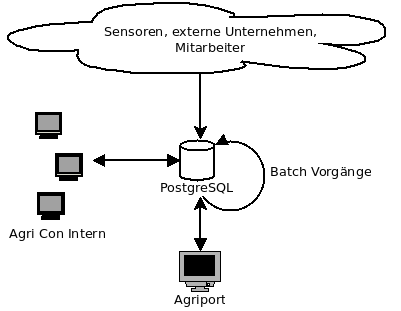
\includegraphics[width=.8\textwidth]{Abbildungen/Ist-Stand.png}
\caption[Aufbau Ist-Stand]{\"{U}bersicht des Aufbaus des Ist-Standes}
\label{fig:iststand}
\end{figure}


- quelldaten benennen und auf Anforderungen verweisen
- Grundschema der DB beschreieben (geografische agratechnische Daten und Daten des Unternehmens, der Organisation)
- Funktionsumfang hinsichtlich berechnung aufzeigen: was macht postgresql und was R
- 
